\section{Resultados y discusión}
\label{sec:resultados_discusion}

Esta sección presenta los resultados obtenidos para los seis experimentos
definidos por

\[
z \in \{4,8\},
\qquad
R \in \{1,2,3\}.
\]

La interpretación distingue entre mínimos globales certificados, cotas
inferiores globales, testigos factibles y óptimos obtenidos dentro de la
familia restringida $2+2+c$.


\subsection{Resultados consolidados}
\label{subsec:resultados_consolidados}

La Tabla~\ref{tab:resultados_consolidados} resume las cotas y los testigos
obtenidos.

\begin{table}[htbp]
    \centering
    \caption{Resultados consolidados para Keccak reducido.}
    \label{tab:resultados_consolidados}
    \begin{tabular}{cccccc}
        \hline
        $z$
        &
        $R$
        &
        Cota inferior
        &
        Cota superior
        &
        Testigo
        &
        Interpretación
        \\
        \hline
        4 & 1 & 1 & 1 & $1$       & Óptimo global \\
        4 & 2 & 4 & 4 & $2+2$     & Óptimo global \\
        4 & 3 & 5 & 13 & $2+2+9$  & Óptimo restringido \\
        8 & 1 & 1 & 1 & $1$       & Óptimo global \\
        8 & 2 & 4 & 4 & $2+2$     & Óptimo global \\
        8 & 3 & 5 & 14 & $2+2+10$ & Óptimo restringido \\
        \hline
    \end{tabular}
\end{table}

En una y dos rondas, la cota inferior coincide con la actividad de un
testigo factible. Por tanto, los valores obtenidos corresponden a mínimos
globales.

En tres rondas, las cotas inferiores y superiores no coinciden. Los
testigos de actividades 13 y 14 son válidos para el problema completo,
pero su optimalidad solo fue demostrada dentro de la familia restringida

\[
2+2+c.
\]


\subsection{Resultados para una ronda}
\label{subsec:resultados_una_ronda}

Para una ronda, la condición

\[
\Delta A_0 \neq 0
\]

y la biyectividad de las transformaciones $\theta$, $\rho$ y $\pi$
garantizan que

\[
\Delta B_0 \neq 0.
\]

Por tanto, al menos una aplicación local de $\chi$ debe recibir una
diferencia no nula:

\[
m_0 \geq 1.
\]

El modelo encontró y reconstruyó testigos que alcanzan exactamente una
S-box activa para ambos tamaños de palabra. En consecuencia,

\[
N_{\mathrm{act}}^{\min}(4,1)
=
N_{\mathrm{act}}^{\min}(8,1)
=
1.
\label{eq:resultado_una_ronda}
\]

La Ecuación~\ref{eq:resultado_una_ronda} constituye un resultado global
exacto.

La igualdad entre $z=4$ y $z=8$ muestra que, en una sola ronda, el aumento
del tamaño del estado no obliga a incrementar la actividad mínima. En
ambas configuraciones existe una diferencia suficientemente localizada
para alcanzar una única posición $(y,k)$ de la capa $\chi$.


\subsection{Resultados para dos rondas}
\label{subsec:resultados_dos_rondas}

Para dos rondas se resolvió el problema auxiliar

\[
m_0+m_1 \leq 3.
\]

CBC demostró la infactibilidad de esta restricción para $z=4$ y $z=8$.
Por tanto, ninguna trayectoria válida puede tener una actividad total
menor o igual que tres.

Paralelamente, se reconstruyeron testigos con distribución

\[
m_0=2,
\qquad
m_1=2.
\]

La actividad total de estos testigos es

\[
m_0+m_1=4.
\]

Al coincidir la cota inferior con la actividad del testigo, se obtiene

\[
N_{\mathrm{act}}^{\min}(4,2)
=
N_{\mathrm{act}}^{\min}(8,2)
=
4.
\label{eq:resultado_dos_rondas}
\]

El patrón

\[
2+2
\]

es, por tanto, óptimo global para ambos tamaños de palabra.

El incremento de una a cuatro S-boxes activas refleja el efecto de la
difusión entre rondas. Aunque una diferencia puede concentrarse en una
única S-box durante la primera aplicación de $\chi$, después de atravesar
una ronda completa no puede conservar una trayectoria total con actividad
menor que cuatro.


\subsection{Resultados para tres rondas}
\label{subsec:resultados_tres_rondas}

Para tres rondas, toda trayectoria válida contiene en sus dos primeras
rondas una trayectoria válida de dos rondas. Como el mínimo global de dos
rondas es cuatro y la diferencia no puede desaparecer antes de la tercera
capa $\chi$, se obtiene

\[
N_{\mathrm{act}}^{\min}(z,3)
\geq
N_{\mathrm{act}}^{\min}(z,2)+1.
\]

Por tanto,

\[
N_{\mathrm{act}}^{\min}(z,3)
\geq
5,
\qquad
z\in\{4,8\}.
\label{eq:cota_inferior_tres_rondas}
\]

La búsqueda exhaustiva restringida a trayectorias $2+2+c$ produjo los
mejores testigos siguientes:

\[
2+2+9=13
\]

para $z=4$, y

\[
2+2+10=14
\]

para $z=8$.

Estos testigos establecen las cotas superiores globales

\[
N_{\mathrm{act}}^{\min}(4,3)
\leq
13
\]

y

\[
N_{\mathrm{act}}^{\min}(8,3)
\leq
14.
\]

En consecuencia, los resultados globales que pueden afirmarse son

\[
5
\leq
N_{\mathrm{act}}^{\min}(4,3)
\leq
13,
\label{eq:resultado_tres_rondas_z4}
\]

y

\[
5
\leq
N_{\mathrm{act}}^{\min}(8,3)
\leq
14.
\label{eq:resultado_tres_rondas_z8}
\]

Los extremos superiores de las
Ecuaciones~\ref{eq:resultado_tres_rondas_z4}
y~\ref{eq:resultado_tres_rondas_z8} corresponden a trayectorias concretas
que satisfacen el modelo completo. Sin embargo, no se demostró que no
existan trayectorias con actividades comprendidas entre las cotas
inferiores y superiores.


\subsection{Resultados de la búsqueda restringida}
\label{subsec:resultados_busqueda_restringida}

Para $z=4$, la búsqueda procesó 200 trayectorias compatibles con actividad
$2+2$. Al evaluar 1024 realizaciones por trayectoria se analizaron

\[
200 \times 1024
=
204\,800
\]

realizaciones concretas. El menor valor obtenido en la tercera ronda fue

\[
c=9.
\]

Para $z=8$, se procesaron 400 trayectorias y

\[
400 \times 1024
=
409\,600
\]

realizaciones. El menor valor obtenido fue

\[
c=10.
\]

Por tanto, dentro de la familia restringida se tiene

\[
\min_{2+2+c} N_{\mathrm{act}}(4,3)
=
13
\]

y

\[
\min_{2+2+c} N_{\mathrm{act}}(8,3)
=
14.
\]

Estas igualdades deben interpretarse exclusivamente dentro del espacio
explorado. Una trayectoria globalmente óptima de tres rondas podría tener
una distribución distinta de

\[
2+2+c.
\]

Por ejemplo, no se descartan mediante esta búsqueda familias con
distribuciones diferentes en las dos primeras rondas, siempre que cumplan
las restricciones completas de propagación.


\subsection{Comparación gráfica}
\label{subsec:comparacion_grafica}

La Figura~\ref{fig:cotas_sboxes} compara las cotas inferiores y superiores
para las seis configuraciones.

\begin{figure}[htbp]
    \centering
    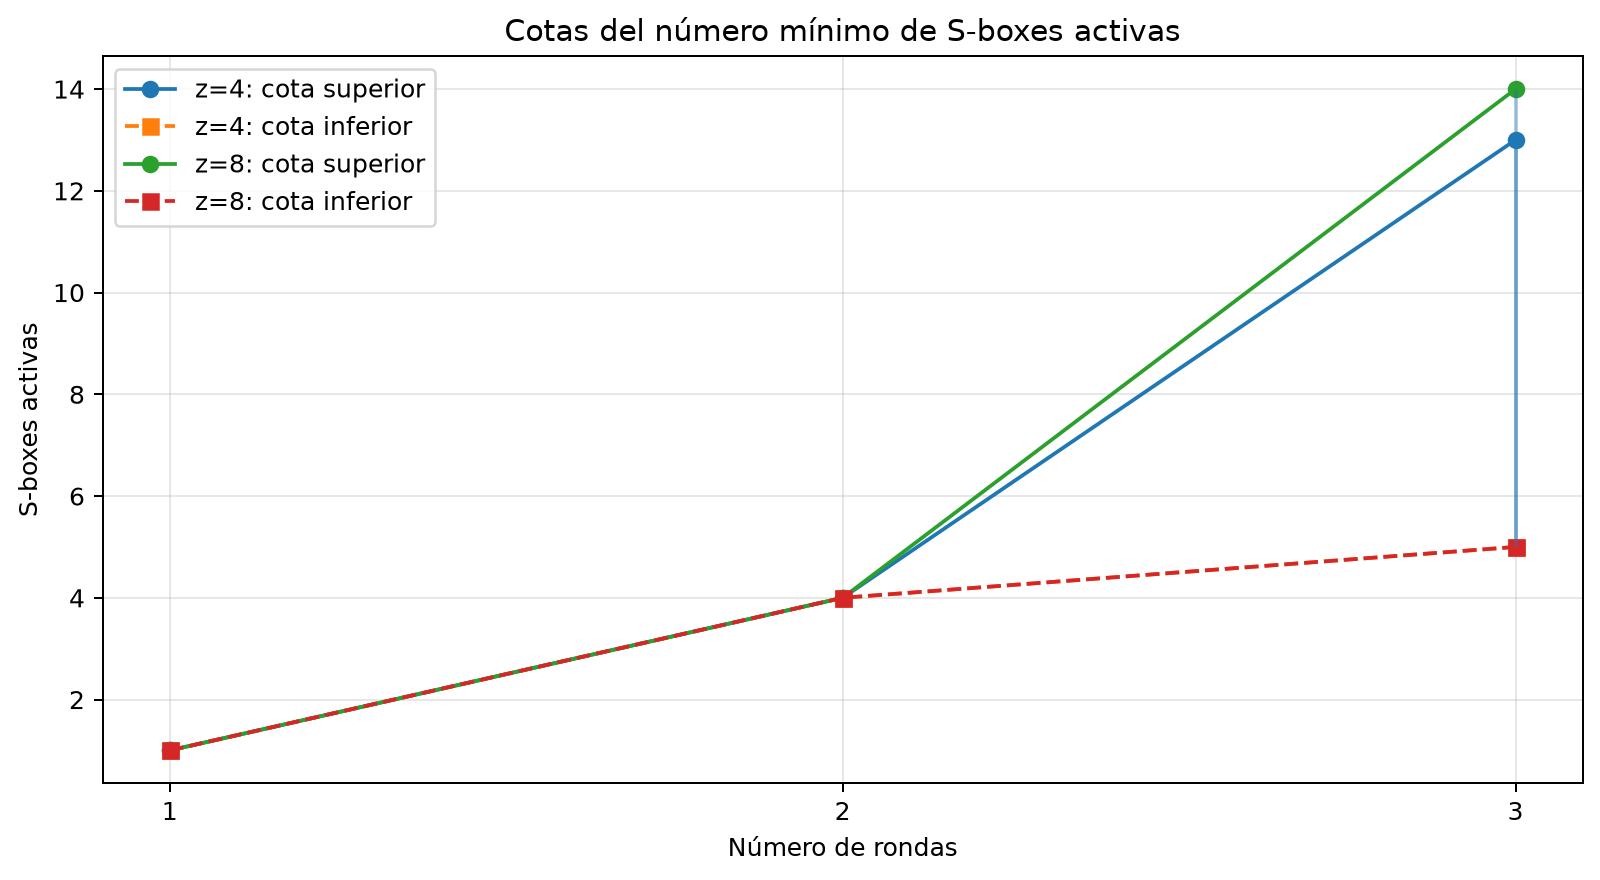
\includegraphics[
        width=0.85\textwidth
    ]{../outputs/figures/active_sbox_bounds.png}
    \caption{Cotas inferiores y superiores del número de S-boxes activas
    para $z=4$ y $z=8$.}
    \label{fig:cotas_sboxes}
\end{figure}

En una y dos rondas, la cota inferior coincide con la cota superior. Esta
coincidencia representa los mínimos globales certificados.

En tres rondas aparece una separación entre ambas cotas. Esta distancia
corresponde a la parte del problema que permanece abierta y no debe
confundirse con la brecha interna de optimalidad informada por CBC.


\subsection{Brecha de certificación}
\label{subsec:brecha_certificacion}

Para describir la amplitud del intervalo disponible se define la brecha de
certificación como

\[
G(z,R)
=
U(z,R)-L(z,R),
\]

donde $L(z,R)$ es la cota inferior global y $U(z,R)$ la actividad del mejor
testigo conocido.

Para tres rondas se obtiene

\[
G(4,3)
=
13-5
=
8,
\]

y

\[
G(8,3)
=
14-5
=
9.
\]

Esta medida expresa la distancia entre las evidencias matemáticas
disponibles. No corresponde a una brecha de optimalidad reportada por el
solver ni permite estimar en qué punto del intervalo se encuentra el
mínimo global.


\subsection{Comparación entre tamaños de palabra}
\label{subsec:comparacion_tamanos}

Los mínimos globales de una y dos rondas son iguales para los dos tamaños
de palabra:

\[
N_{\mathrm{act}}^{\min}(4,1)
=
N_{\mathrm{act}}^{\min}(8,1),
\]

\[
N_{\mathrm{act}}^{\min}(4,2)
=
N_{\mathrm{act}}^{\min}(8,2).
\]

Esta igualdad indica que, para los horizontes estudiados, duplicar la
longitud de palabra y el número de aplicaciones locales de $\chi$ por
ronda no obliga a incrementar el mínimo global.

En tres rondas, los mejores testigos restringidos presentan una diferencia
de una S-box:

\[
13
\quad \text{para } z=4,
\]

frente a

\[
14
\quad \text{para } z=8.
\]

No obstante, esta diferencia no demuestra que el mínimo global aumente con
$z$. Las cotas inferiores permanecen iguales y los extremos superiores
provienen de una familia restringida. Por tanto, no puede establecerse una
relación general entre el tamaño de palabra y la actividad mínima de tres
rondas.


\subsection{Interpretación criptanalítica}
\label{subsec:interpretacion_criptanalitica}

Los resultados muestran tres comportamientos principales:

\begin{enumerate}
    \item \textbf{Localización en una ronda.}
    Una diferencia inicial no nula puede alcanzar una única aplicación
    local de $\chi$.

    \item \textbf{Difusión en dos rondas.}
    La interacción entre las capas lineales y no lineales eleva el mínimo
    global a cuatro S-boxes activas.

    \item \textbf{Mayor dispersión en tres rondas.}
    Las mejores extensiones encontradas dentro de la familia $2+2+c$
    activan nueve o diez S-boxes adicionales en la tercera ronda.
\end{enumerate}

El conteo de S-boxes activas mide cuántos componentes no lineales reciben
una diferencia, pero no determina la probabilidad completa de una
característica diferencial. Dos trayectorias con la misma actividad pueden
presentar diferentes transiciones locales y, por tanto, probabilidades
distintas.

Para obtener una evaluación diferencial más completa sería necesario
incorporar los pesos de las transiciones de $\chi$ y analizar su
compatibilidad a lo largo de las rondas. En el alcance de este trabajo,
la actividad se interpreta como una medida estructural de difusión no
lineal.


\subsection{Síntesis de los resultados}
\label{subsec:sintesis_resultados}

Los seis experimentos pueden resumirse mediante

\[
N_{\mathrm{act}}^{\min}(4,1)=1,
\qquad
N_{\mathrm{act}}^{\min}(4,2)=4,
\qquad
5
\leq
N_{\mathrm{act}}^{\min}(4,3)
\leq
13,
\]

y

\[
N_{\mathrm{act}}^{\min}(8,1)=1,
\qquad
N_{\mathrm{act}}^{\min}(8,2)=4,
\qquad
5
\leq
N_{\mathrm{act}}^{\min}(8,3)
\leq
14.
\]

Los resultados de una y dos rondas son mínimos globales. Los resultados de
tres rondas son intervalos formados por una cota inferior global y una cota
superior respaldada por un testigo concreto.

Los valores 13 y 14 son óptimos dentro de la familia $2+2+c$, pero no se
presentan como mínimos globales del espacio completo de tres rondas.